\section{TIC en la educación}
\setcounter{sectiontotal}{3}

\begin{frame}
    \frametitle{\pagetitle}
    \framesubtitle{Corrientes pedagógicas}

    \pause{}
\begin{columns}
\column{.4\textwidth} \hspace{0.5cm}
\begin{overprint}
    \onslide<2|handout:1> 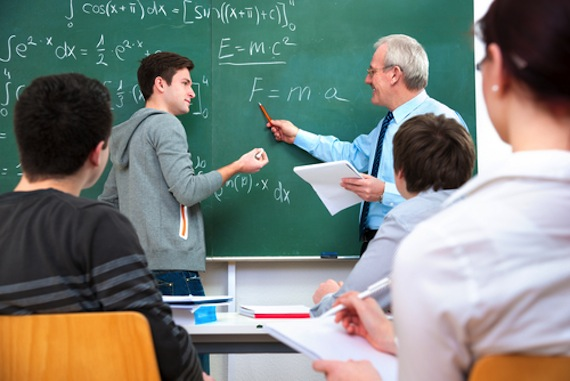
\includegraphics[width=\textwidth, height=5.5cm]{imagenes/instruccionismo} 
    \onslide<3|handout:0> 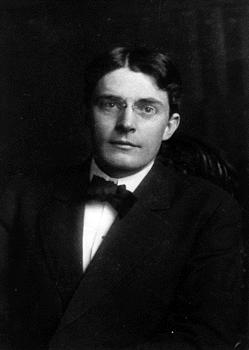
\includegraphics[width=\textwidth, height=5.5cm]{imagenes/conductismo} 
    \onslide<4|handout:0> 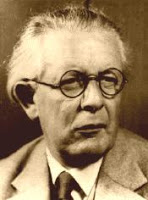
\includegraphics[width=\textwidth, height=5.5cm]{imagenes/constructivismo} 
    \onslide<5|handout:0> 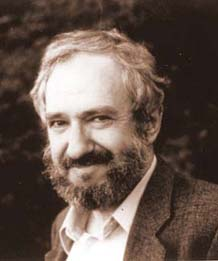
\includegraphics[width=\textwidth, height=5.5cm]{imagenes/construccionismo} 
\end{overprint}

\column{.7\textwidth} \hspace{0.5cm}
\begin{itemize}[<+->]
	\item Instruccionismo
	\item Conductismo
	\item Constructivismo
	\item Construccionismo
\end{itemize}
\end{columns}


\end{frame}

\begin{frame}
    \frametitle{\pagetitle}
    \framesubtitle{Ventajas}
    \begin{itemize}[<+->]
        \item Nuevos modelos pedagógicos
        \item Eliminación de distancias
        \item Colaboración distribuida
        \item Motivación para aprender
        \item Adquisición de habilidades básicas
    \end{itemize}
\end{frame}

\begin{frame}
    \frametitle{\pagetitle}
    \framesubtitle{Desafíos}
	 \begin{itemize}[<+->]
        \item Falta de motivación de los profesionales
        \item Altas expectativas
        \item Brecha social
        \item Aspectos financieros
    \end{itemize}
\end{frame}
